%%%%%%%%%%%%%%%%%%%%%%%%%%%%%
\subsection{Project Overview}
%%%%%%%%%%%%%%%%%%%%%%%%%%%%%
% Student provides a high-level overview of the project in layman’s terms. Background information such as the problem domain, the project origin, and related datasets or input data is given.

In layman terms, Machine learning consists of programming the computer to learn from previous data. Today, Machine Learning's method, Deep Reinforcement Learning, is gaining popularity since lots of applications has been given to it, such as Video Games, unmanned vehicles, and control systems. The latter is a well-known field where the goal is to make dynamical systems behave in a desired manner, to achieve this it is required to obtain the mathematical model of the system as explained in \cite{Control}

Since control systems are dynamic, all its environments are modeled as a continuous state space and most of the times as a continuous action space as well. Therefore, it signifies a challenging task to solve by machine learning, some of the algorithms able to tackle these problems are deep Q learning (for infinite state spaces and discrete action spaces), and actor-critic methods (for infinite state and action spaces), both of them being from Deep Reinforcement Learning field. 

In many cases it is not possible to know all the system's features thus it is not possible to get the mathematical model of the system, that is where Deep Reinforcement Learning came in place. There are lots of works developed in Control Systems related to Reinforcement learning. For instance, one approach of Reinforcement Learning applied to Control systems is presented in "A heuristic approach to reinforcement learning control systems" \cite{1098193}

%%%%%%%%%%%%%%%%%%%%%%%%%%%%%%
\subsection{Problem Statement}
%%%%%%%%%%%%%%%%%%%%%%%%%%%%%%
% The problem which needs to be solved is clearly defined. A strategy for solving the problem, including discussion of the expected solution, has been made.

The project aims to solve an OpenAI gym environment from the control section that can be seen here \href{https://gym.openai.com/envs/#classic_control}{Control Environments}. The environment selected is the MountainCar-v0 because it has a continuous state space with a deterministic action space being a good candidate for applying deep q learning. The details of the problem are as follows:
\begin{itemize}
\item \textbf{Task:} MountainCar-v0
\item \textbf{Category:} Classic Control
\item \textbf{Goal:} Get an under powered car to the top of a hill (top = 0.5 position) by creating momentum as shown in Fig.\ref{fig:car}
\begin{figure}[h]
\centering
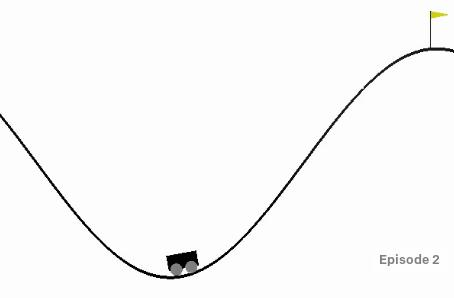
\includegraphics[width=0.8\textwidth]{environment.jpg}
\caption{\label{fig:car} Mountain Car environment}
\end{figure}

\item \textbf{Termination Criteria:} The episode ends when either the goal is reached or 200 actions are made.
\item \textbf{Rewards:} -1 penalty for each environment step until the termination criteria is met.

\item \textbf{Initial state:} The environment starts with the car randomly positioned between -0.6 and -0.4 and always with a velocity of 0.
\item \textbf{Potential Solution:} Since the environment has continuous state space and discrete action space, a good candidate would be a \textbf{Deep Q Network}
\item \textbf{Solution Concerns:} The car will eventually find a solution, however, in order to get an optimal policy in fewer episodes, it might be required to implement Double Deep Q Learning or prioritized memory.

\end{itemize}


%%%%%%%%%%%%%%%%%%%%
\subsection{Metrics}
\label{sub:Metrics}
%%%%%%%%%%%%%%%%%%%%
% Metrics used to measure performance of a model or result are clearly defined. Metrics are justified based on the characteristics of the problem.

\textbf{Average Reward} The main metric for the project will be the average reward in 100 consecutive episodes. The reason to take 100 rewards averaged is to avoid the model to work just for certain specific states in the environment. 
\newline
\textbf{Number of episodes} The secondary metric is the number of episodes in which the problem converges to a solution.

% add here: Why you have chosen to use the 100 episode average performance? Why average them? Why not just choose the 'best'?
